% ---
% Capa
% ---
\imprimircapa
% ---

% ---
% Folha de rosto
% (o * indica que haverá a ficha bibliográfica)
% ---
\imprimirfolhaderosto*
% ---

% ---
% Inserir a ficha bibliografica
% ---
\begin{fichacatalografica}
	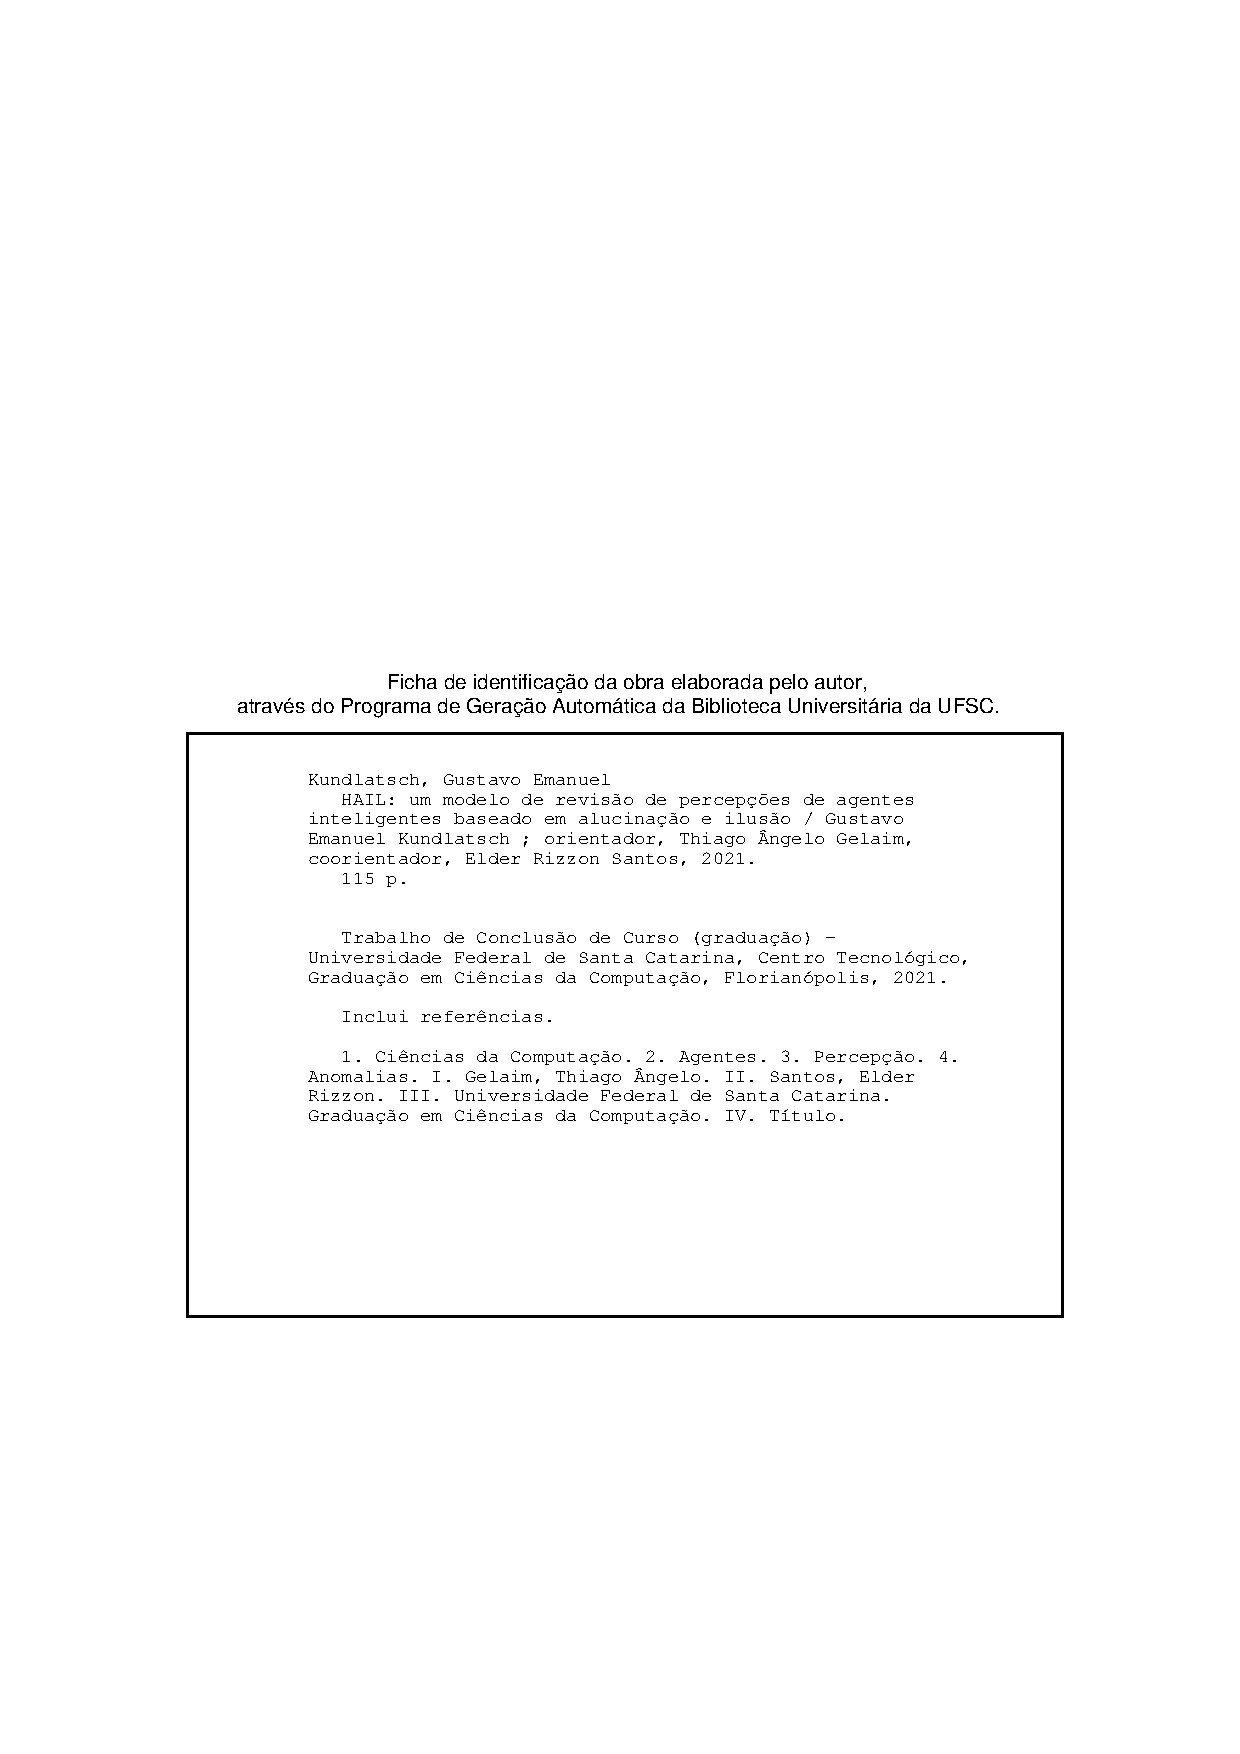
\includepdf{beforetext/Ficha_Catalografica.pdf}
\end{fichacatalografica}
% ---

% ---
% Inserir folha de aprovação
% ---
\begin{folhadeaprovacao}
	\OnehalfSpacing
	\centering
	\imprimirautor\\%
	\vspace*{10pt}		
	\textbf{\imprimirtitulo}%
	\ifnotempty{\imprimirsubtitulo}{:~\imprimirsubtitulo}\\%
	%		\vspace*{31.5pt}%3\baselineskip
	\vspace*{\baselineskip}
	%\begin{minipage}{\textwidth}
	O presente trabalho em nível de \imprimirnivel~foi avaliado e aprovado por banca examinadora composta pelos seguintes membros:\\
	%\end{minipage}%
	\vspace*{\baselineskip}
	Dr. Thiago Ângelo Gelaim\\
	Orientador\\
	\vspace*{\baselineskip}
	Prof. Dr. Elder Rizzon Santos \\
	Coorientador e Responsável\\
	\vspace*{\baselineskip}
	Prof. Dr. Rafael de Santiago\\
	\vspace*{\baselineskip}
	Me. Rodrigo Rodrigues Pires de Mello\\
	\vspace*{2\baselineskip}
	\begin{minipage}{\textwidth}
		Certificamos que esta é a \textbf{versão original e final} do trabalho de conclusão que foi julgado adequado para obtenção do título de \imprimirformacao.\\
	\end{minipage}
	%    \vspace{-0.7cm}
	\vspace*{\fill}
	\assinatura{\OnehalfSpacing Coordenação do Programa de Graduação}
	\vspace*{\fill}
	\assinatura{\OnehalfSpacing\imprimirorientador \\ \imprimirorientadorRotulo}
	%	\ifnotempty{\imprimircoorientador}{
	%	\assinatura{\imprimircoorientador \\ \imprimircoorientadorRotulo \\
	%		\imprimirinstituicao~--~\imprimirinstituicaosigla}
	%	}
	% \newpage
	\vspace*{\fill}
	\imprimirlocal, \imprimirano.
\end{folhadeaprovacao}
% ---

% ---
% Dedicatória
% ---
\begin{dedicatoria}
	\vspace*{\fill}
	\noindent
	\begin{adjustwidth*}{}{5.5cm} 
		\raggedleft       
		Para meus pais, que sempre souberam que o melhor investimento para os filhos é a educação.
	\end{adjustwidth*}
\end{dedicatoria}
% ---

% ---
% Agradecimentos
% ---
\begin{agradecimentos}

    Quando fazemos uma escolha, ela recebe o peso de toda a potencialidade morta das alternativas que não foram escolhidas. Sou muito grato a minha família, que sempre me deu toda a liberdade do mundo para tomar minhas próprias escolhas e que também sempre me apoiou, no acerto ou no erro, independente da dificuldade enfrentada. Eu escolhi cursar computação, e mesmo que minha família não entenda muito bem o que isso significa, sempre esteve comigo me incentivando a seguir meus sonhos.

	Este trabalho não representa o ciclo final de minha graduação, mas todo o caminho trilhado nesses anos de curso. Ele é resultado de um processo que começou no fim do meu primeiro semestre, um processo que me fez conhecer muitas pessoas incríveis e que me desenvolveu tanto profissionalmente quanto como pessoa. O laboratório sempre foi para mim uma forma de expressar minha criatividade, e esta monografia é resultado de apenas uma das muitas ideias que eu tive. Por essa liberdade de criar e por todas as reuniões de orientação que tive ao longo desses anos eu agradeço ao professor Elder e ao Thiago, que tiveram a paciência de me acolher na minha iniciação científica.
	
	A maior benção que recebi na vida foram meus amigos, e não posso deixar de agradecê-los aqui. Seja para jogar, reclamar da vida, chorar as mágoas ou simplesmente desfrutar da companhia uns dos outros, meus amigos nunca me deixaram na mão. Eu sempre quis ser um contador de histórias, e compartilhar meus causos com meus amigos, distribuindo sorrisos e gargalhadas, é algo que dinheiro nenhum no mundo seria capaz da comprar.
	
	Por fim, gostaria de agradecer cada servidor da UFSC e profissional da comunidade, que são responsáveis pela alimentação, limpeza e organização de nossa universidade pública e gratuita. Sem o trabalho de cada uma dessas pessoas, essa conquista não seria possível.

\end{agradecimentos}
% ---

% ---
% Epígrafe
% ---
\begin{epigrafe}
	\vspace*{\fill}
	\begin{flushright}
		\textit{``Qualquer lugar é o paraíso desde que queira viver.\\
		    Afinal, todos estão vivos.\\
		    E, enquanto for assim, todos têm chance de ser feliz.''\\
			(Anno, End of Evangelion, 1997)}
	\end{flushright}
\end{epigrafe}
% ---

% ---
% RESUMOS
% ---

% resumo em português
\setlength{\absparsep}{18pt} % ajusta o espaçamento dos parágrafos do resumo
\begin{resumo}
	\SingleSpacing
	Percepções são a principal maneira de uma entidade receber informações do ambiente. Cada pessoa possui uma maneira diferente de perceber e interpretar o mundo. Entretanto, sabe-se que na percepção humana existem anomalias, que são percepções incorretas que enganam a mente. Dito isso, como podemos saber se nossas percepções são reais ou se são apenas fruto de nossa imaginação? E a questão derivada disso é: e computadores? Agentes inteligentes são entidades computacionais autônomas capazes de tomar decisões baseadas no ambiente no qual estão inseridos, e utilizam sensores para reconhecerem o mundo a sua volta. Mas esses sensores podem falhar. Neste trabalho, apresentamos um modelo genérico de revisão de percepções, capaz de tratar anomalias recebidas pelo agente e criar novos planos a partir delas para se adaptar ao ambiente. Esse modelo foi implementado e submetido a experimentos para testar seu funcionamento. As simulações realizadas demonstraram que o modelo é capaz de detectar e classificar as anomalias, e que em ambientes com grande quantidade de percepções inválidas o modelo consegue ter maior impacto criando novos planos através do planejamento automatizado e aumentando a quantidade de percepções válidas recebidas pelo raciocínio do agente.
	
	\textbf{Palavras-chave}: Agentes. Percepção. Anomalias.
\end{resumo}

% resumo em inglês
\begin{resumo}[Abstract]
	\SingleSpacing
	\begin{otherlanguage*}{english}
		Perceptions are the primary way for an entity to receive information from the environment. Each person has a different manner of percept and interpret the world. However, it is known that in human perception, there are anomalies, incorrect perceptions that deceive the mind. So, how can we know if our perceptions are real or just tricks from our minds? Furthermore, the follow-up question is: what about computers? Intelligent agents are computational entities capable of making decisions based on the environment and use sensors to perceive the world. However, sensors can fail. In the current work, we present a generic model of perception revision, capable of treating anomalies received by the agent and creating new plans to adapt to the environment. This model was implemented and submitted to experiments to test its behaviour. The simulations demonstrate that the model is capable of detecting and classifying anomalies. In environments with a high amount of invalid perceptions, the model can have more impact creating new plans through the automatic planning process and increasing the number of valid perceptions received by the agent's cognition.
		
		\textbf{Keywords}: Agents. Perception. Anomalies.
	\end{otherlanguage*}
\end{resumo}
%% resumo em francês 
%\begin{resumo}[Résumé]
% \begin{otherlanguage*}{french}
%    Il s'agit d'un résumé en français.
% 
%   \textbf{Mots-clés}: latex. abntex. publication de textes.
% \end{otherlanguage*}
%\end{resumo}
%
%% resumo em espanhol
%\begin{resumo}[Resumen]
% \begin{otherlanguage*}{spanish}
%   Este es el resumen en español.
%  
%   \textbf{Palabras clave}: latex. abntex. publicación de textos.
% \end{otherlanguage*}
%\end{resumo}
%% ---

{%hidelinks
	\hypersetup{hidelinks}
	% ---
	% inserir lista de ilustrações
	% ---
	\pdfbookmark[0]{\listfigurename}{lof}
	\listoffigures*
	\cleardoublepage
	% ---
	
	% ---
	% inserir lista de quadros
	% ---
	\pdfbookmark[0]{\listofquadrosname}{loq}
	\listofquadros*
	\cleardoublepage
	% ---
	
	% ---
	% inserir lista de tabelas
	% ---
	\pdfbookmark[0]{\listtablename}{lot}
	\listoftables*
	\cleardoublepage
	% ---
	
	
	% ---
	% inserir lista de abreviaturas e siglas (devem ser declarados no preambulo)
	% ---
	% ---------------------------------------------------
% ------ Lista de abreviaturas e siglas -------------
% ---------------------------------------------------

\begin{siglas}
  \item[ BDI ] \hspace{0.7cm} \emph{Belief-Desire-Intention}
  \item[ EOM ] \hspace{0.7cm} \textit{Environment Object Model}
  \item[ IA ] \hspace{0.7cm} Inteligência Artificial
  \item[ K-CoPMan ] \hspace{0.4cm} \textit{Knowledge enabled Cognitive Perception for Manipulation}
  \item[ NPC ] \hspace{0.7cm} Número de Percepções recebidas por Ciclo
  \item[ OA-SMTRNN ] \textit{Object Augmented Supervised Multiple Timescale Recurrent}
  
  \hspace{0.7cm} \textit{Neural Network}
  \item[ PDDL ] \hspace{0.7cm} \textit{Planning Domain Definition Language}
  \item[ PMK ] \hspace{0.7cm} \textit{Perception and Manipulation Knowledge}
  \item[ PPI ] \hspace{0.7cm} Porcentagem de Percepções Inválidas
  \item[ RP ] \hspace{0.7cm} Relação Percentual
  \item[ SMA ] \hspace{0.7cm} Sistema Multiagente
  \item[ TMA ] \hspace{0.7cm} Tempo Médio gasto pelo planejamento Automatizado
  \item[ TMC ] \hspace{0.7cm} Tempo Médio gasto em um Ciclo de raciocínio
\end{siglas}
	% ---
	
	% ---
	% inserir lista de símbolos (devem ser declarados no preambulo)
	% ---
	% ---------------------------------------------------
% ----------- Lista de símbolos ---------------------
% ---------------------------------------------------

\begin{simbolos}
  \item[$ \Delta $] Função de transição do modelo de revisão de percepções
  \item[$ \Gamma $] Função de transição que especifica um sistema de transição de estados $\Sigma$
  \item[$ \gamma $] Função de percepção do agente
  \item[$ \theta $] Função de refinamento
  \item[$ \rho $] Conjunto de percepções refinadas
  \item[$ \Sigma $] Sistema de transição de estados de um modelo conceitual de planejamento automatizado
  \item[$ \Psi $] Conjunto união formado pelas pré-condições das ações que compõem um plano
  \item[$ \psi $] Conjunto de pré-condições de uma ação
  \item[$ \Omega $] Conjunto união formado pelas pós-condições das ações que compõem um plano
  \item[$ \omega $] Conjunto de pós-condições de uma ação
  \item[$ A $] Conjunto finito ou recursivamente enumerável de ações
  \item[$ Ab $] Conjunto de blocos avaliadores
  \item[$ Ab_{h} $] Bloco avaliador de alucinações
  \item[$ Ab_{i1} $] Bloco avaliador de ilusões classe 1
  \item[$ Ab_{i2} $] Bloco avaliador de ilusões classe 2
  \item[$ Ag$ ] Agente
  \item[$ Ap $] Conjunto de blocos de planejamento automatizado
  \item[$ Ap_{h} $] Bloco de planejamento automatizado de alucinações
  \item[$ Ap_{i} $] Bloco de planejamento automatizado de ilusões
  \item[$ c $] Contexto do agente
  \item[$ Ce $] Função equação de limpeza do bloco avaliador
  \item[$ Cf $] Função de limpeza do bloco avaliador
  \item[$ D $] Conjunto de decisores
  \item[$ d_{a} $] Decisor de anomalias
  \item[$ d_{h} $] Decisor de alucinações
  \item[$ d_{i} $] Decisor de ilusões
  \item[$ E $] Conjunto finito ou recursivamente enumerável de eventos
  \item[$ K $] Conjunto de conhecimentos do agente
  \item[$ L $] Lista ordenada
  \item[$ |L| $] Número de elementos de uma lista ordenada
  \item[$ L_i $] Elemento $i$ da lista ordenada $L$
  \item[$ M_{ai} $] Módulo de alucinação e ilusão
  \item[$ P $] Conjunto de planos do agente
  \item[$ p $] Conjunto de percepções iniciais
  \item[$ P(L_i) $] Função peso da lista ponderada
  \item[$ Pf $] Função de processamento do bloco avaliador
  \item[$ S $] Conjunto finito ou recursivamente enumerável de estados
  \item[$ T_{m}(x) $] Função tempo médio de x
  \item[$ W $] Função peso de uma anomalia
  \item[$ Z $] Descrição de sistema
\end{simbolos}


	% ---
	
	% ---
	% inserir o sumario
	% ---
	\pdfbookmark[0]{\contentsname}{toc}
	\tableofcontents*
	\cleardoublepage
	
}%hidelinks
% ---